% IEEE standard conference template; to be used with:
%   spconf.sty  - LaTeX style file, and
%   IEEEbib.bst - IEEE bibliography style file.
% --------------------------------------------------------------------------

\documentclass[letterpaper]{article}
\usepackage{spconf,amsmath,amssymb,graphicx}
\usepackage{array}
\usepackage{nicematrix}
\usepackage{tikz}
\usepackage{graphicx}
\usepackage{caption}
\usepackage{pdfpages}

% Example definitions.
% --------------------
% nice symbols for real and complex numbers
\newcommand{\R}[0]{\mathbb{R}}
\newcommand{\C}[0]{\mathbb{C}}

% bold paragraph titles
\newcommand{\mypar}[1]{{\bf #1.}}

% Title.
% ------
\title{Parallelizing the Smith-Waterman algorithm for genome sequencing}
%
% Single address.
% ---------------
\name{Kosta Stojiljkovic, Han Yao Choong, Langwen Huang, Benjamin Langer} 
\address{Progress report - Design of Parallel and High-Performance Computing - Group 15}

% For example:
% ------------
%\address{School\\
%		 Department\\
%		 Address}
%
% Two addresses (uncomment and modify for two-address case).
% ----------------------------------------------------------
%\twoauthors
%  {A. Author-one, B. Author-two\sthanks{Thanks to XYZ agency for funding.}}
%		 {School A-B\\
%		 Department A-B\\
%		 Address A-B}
%  {C. Author-three, D. Author-four\sthanks{The fourth author performed the work
%		 while at ...}}
%		 {School C-D\\
%		 Department C-D\\
%		 Address C-D}
%

\begin{document}
%\ninept
%
\maketitle
%

\section{Introduction}

Genome sequencing has become a promising field tool that is hypothesized to facilitate researchers to find the root cause (and subsequently the cure) for a number of genetic diseases in the future. Of central concern for this ambitious task is the similarity between two sequence portions (effectively two strings). Finding an a close alignment of two sequences indicates to a researcher the possibility of a mutation. The Smith-Waterman algorithm was originally invented for that purpose and different (usually heuristic) variations of it power standard software such as BLAST and FASTA \cite{Maekinen.2015}.

% Diviation from proposal
The investigation into three different algorithms listed in the initial proposal (see attached below) was discarded in favor of a more thorough and deeper look into a single one of them (namely Smith-Waterman). From a computer science perspective all of these algorithms are rather similar, consequently the team decided to focus its efforts on the one which is most relevant in the given domain.

\section{Parallelization strategy}
In our first attempts two different strategies were pursued that either exploit the inherent structure of the problem or the overall nature of the problem.

\mypar{Fine-grained approach} A major step of the Smith-Waterman algorithm is the calculation of a similarity matrix which measure how closely parts of the tow sequences resemble each other. Each entry in the matrix depends only on its neighbors to the west, north, and north-west. For example, calculating the value encircled in red in Figure 1 only depends on the black encircled entries. Exploiting these data dependencies, each anti-diagonal in the similarity matrix may be calculated independently from each other. This is general approach taken by a number of papers \cite[Sec. 2]{Chen.2010}. We plan to run our benchmark also against those projects as soon as a more representative test example is determined.

The current implementation utilizes OpenMP to split calculations along the anti-diagonal among multiple cores.

\setlength{\extrarowheight}{1.5mm}
\begin{figure}
	\centering
	$\begin{pNiceMatrix}%
		[name=mymatrix,
		first-col,
		first-row,
		columns-width = 0.3cm
		]
		&   & \mathbf{T} & \mathbf{G} & \mathbf{T} & \mathbf{T} \\
		& 0 & 0 & 0 & 0 & 0 \\
		\mathbf{G} & 0 & 0 & 3 & 1 & 0 \\
		\mathbf{G} & 0 & 0 & 3 & 1 & 0 \\
		\mathbf{T} & 0 & 3 & 1 & 6 & 4 \\
		\mathbf{T} & 0 & 3 & 1 & 4 & 9 \\
		
	\end{pNiceMatrix}$
	\begin{tikzpicture}[remember picture,overlay]
		\draw[line width=0.25mm, red](mymatrix-4-4)circle (2mm);
		\draw[line width=0.25mm](mymatrix-3-4)circle (2mm);
		\draw[line width=0.25mm](mymatrix-4-3)circle (2mm);
		\draw[line width=0.25mm](mymatrix-3-3)circle (2mm);
	\end{tikzpicture}
	\caption{Data dependencies between entries}
\end{figure}%



\mypar{Coarse-grained approach} Usually researchers are not solely interested in how one particular sequence can be aligned optimally to another. Biologically more interesting is the comparison of one  sequence towards a large reference database. For this purpose, we split our mock library file among MPI (message passing interface) nodes and let each one run the algorithm separately. This task is insofar optimal for parallel computers as that no communication between nodes is ever necessary with the exception of generating the output file.



\section{Work split}



\begin{center}
	\begin{tabular}{ | m{1.5cm} | m{6cm} | } 
		\hline
		Name & Main focus* \\ 
		\hline
		Kosta & Coarse-grain approach, MPI \\ 
		Langwen & CMake setup, Matrix transformation \\ 
		Han & Bioinf input, OpenMP \\
		Benjamin & Testing, base algorithm implementation \\
		\hline
	\end{tabular}
\end{center}
*Various teammates also contributed actively and significantly to other fields.



% References should be produced using the bibtex program from suitable
% BiBTeX files (here: bibl_conf). The IEEEbib.bst bibliography
% style file from IEEE produces unsorted bibliography list.
% -------------------------------------------------------------------------
\bibliographystyle{IEEEbib}
\bibliography{bibl_conf}

\clearpage

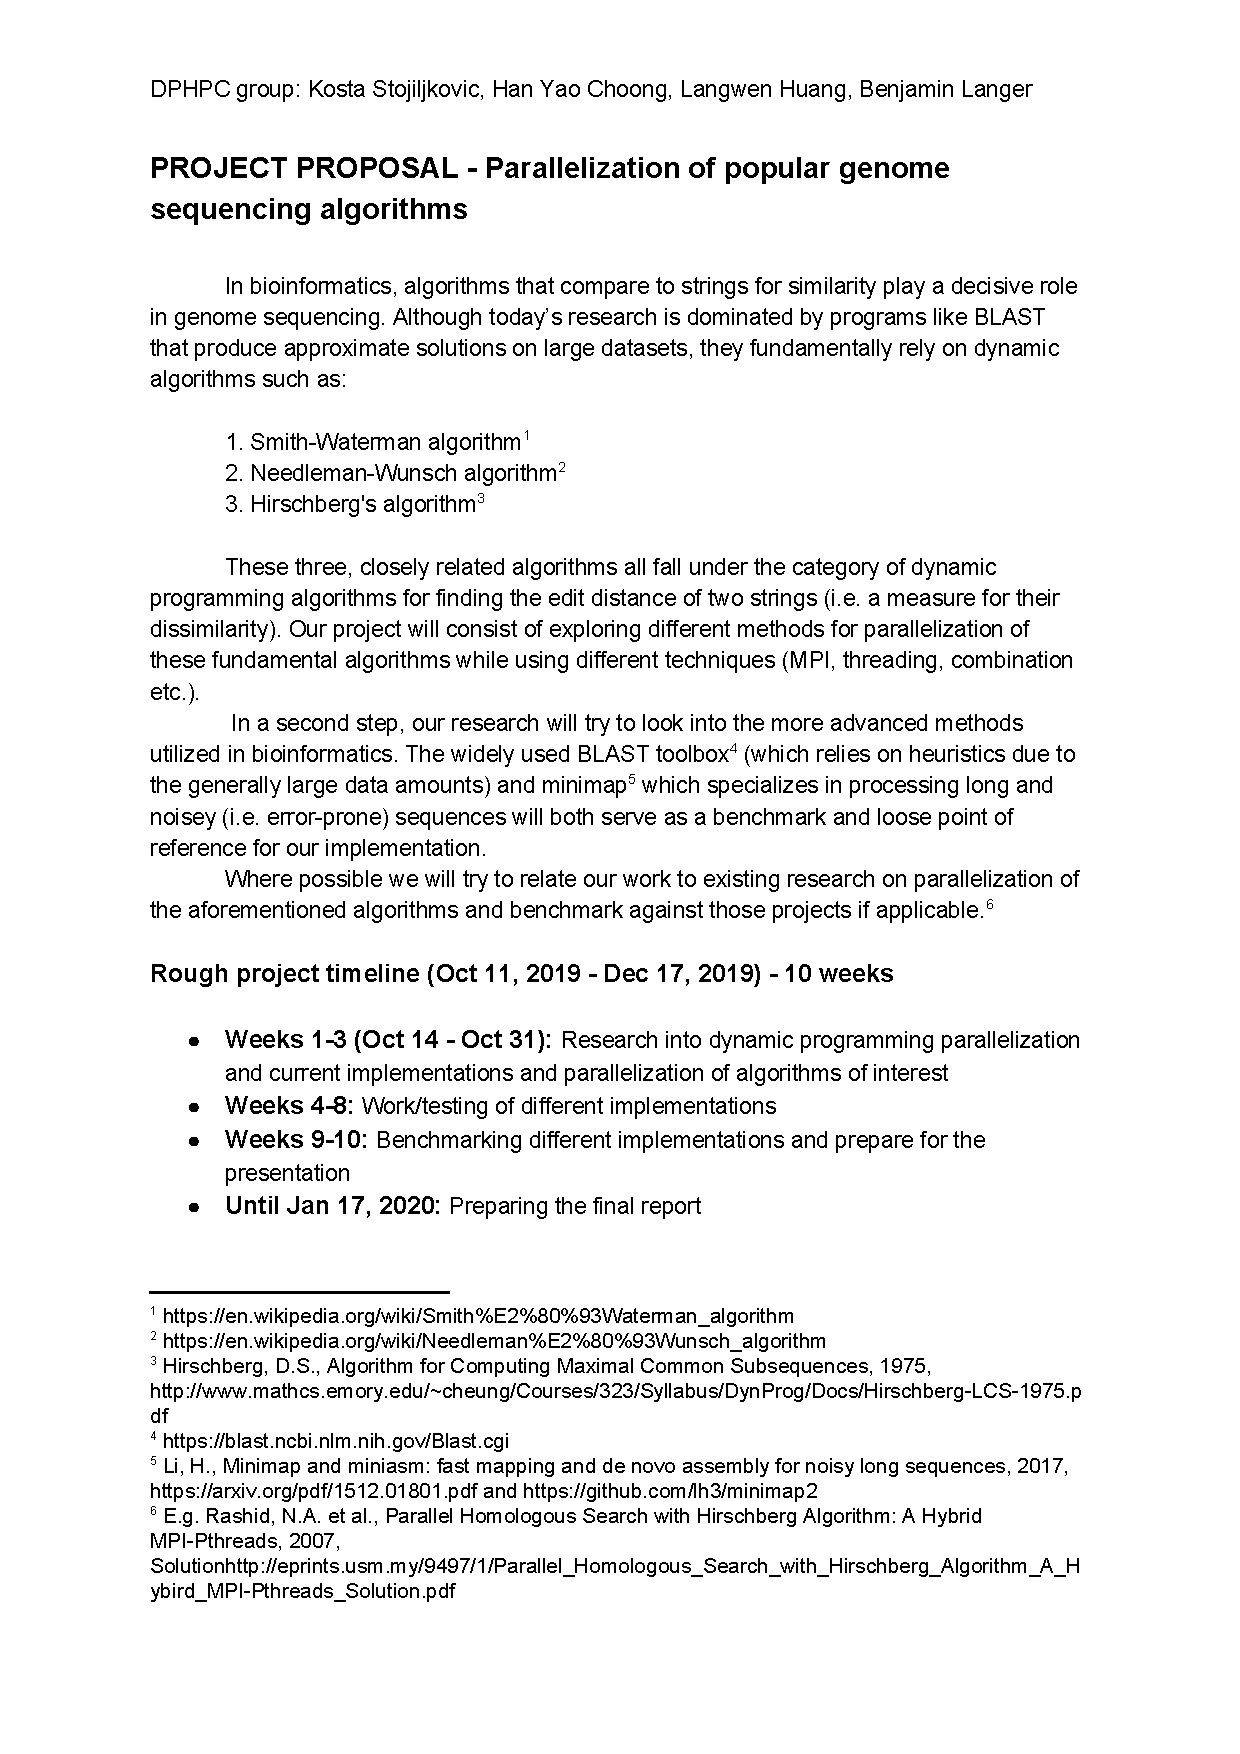
\includepdf{../proposal/DPHPC_proposal.pdf}

\end{document}

